\documentclass[a4paper, 12pt]{article}

\usepackage{amsmath,amsfonts,graphicx} %math packages
\usepackage{listings,xcolor} %code snippet packages
\usepackage{setspace} %allows spaces to be set
\usepackage{tabularx} %flexible width tables
\usepackage{multicol} %enables multiple columns
\usepackage{enumitem} %customized lists
\usepackage[skip=10pt]{parskip} %flexible paragraph spacing options
\usepackage[ruled,vlined,linesnumbered]{algorithm2e}
\SetKwInOut{Input}{Input}
\SetKwInOut{Output}{Output}
% graphicx is required for images
\usepackage{graphicx}
\usepackage{tikz}
\usepackage{csquotes} %quotations

\title{ANN with SegTree and Constant Weight PIR}
\author{Ray Wang, Florian Kerschbaum}
\date{\today}

\setlength{\parindent}{0pt} %remove leading space in paragraphs
\pagestyle{empty} %empties the heading and footer 

\begin{document}
\pagenumbering{gobble} %remove page numbers from title page
\maketitle %add titlepage
\newpage

\pagenumbering{arabic} %reset page numbering to default 
\section{Introduction}
Previous 
% define ANN link high-dimension ANN paper,  

Fix a \(d\) dimensional vector space over \(R\), and a set of feature vectors \(P\). 
we describe a \((c,r)-ANN\) datastructure with time-complexity \(T\)
space complexity \(S\) such that 
\begin{align*}
  T \in O(d|P|) \qquad \text{and} \qquad S \in O(\log(|P|) + \log{d})
\end{align*}
for 

\begin{center}
\begin{tikzpicture}[
  level distance=45 pt,
  every node/.style={circle,draw}, % nodes are circles
  level 1/.style={sibling distance=200 pt},
  level 2/.style={sibling distance=100 pt},
  level 3/.style={sibling distance=60 pt}
]
  \node {R}
    child {node {} 
      child {node {}
        child {node {0}{}}
        child {node {1}{}}
      }
      child {node {}
        child {node {2}{}}
        child {node {3}{}}
      }
    }
    child {node {} 
      child {node {}
        child {node {4}{}}
        child {node {5}{}}
      }
      child {node {}
        child {node {6}{}}
        child {node {7}{}}
      }
    }
  ;
\end{tikzpicture}
\end{center}
Suppose there is a query for a vector in bucket \(3\) 
who's nearest neighbour is in bucket \(4\). 
With this segment tree, the result will be a vector in \(R\), the root.
This is too inaccurate, so we propose a method to imporve this bound. 
In fact, for any query vector \(q\) with nearest neighbour a distance \(r\) units away,
the vector we return from the algorithm is no more than \(8\sqrt{d}r\). 

Method: build the standard quantization tree over \(B\) buckets. 
Let the tree have height \(h = \lfloor \log_2(B+1)\rfloor \).
Define the root to be on level \(0\). 
For each level \(0 \leq l < h-1 \), define a sequence of offset integers 
\begin{align*}
  o_{l} = 2^{h-l-1}-1 
\end{align*}
Define \(o_{h-1} = 0 \). Then 



\begin{center}
  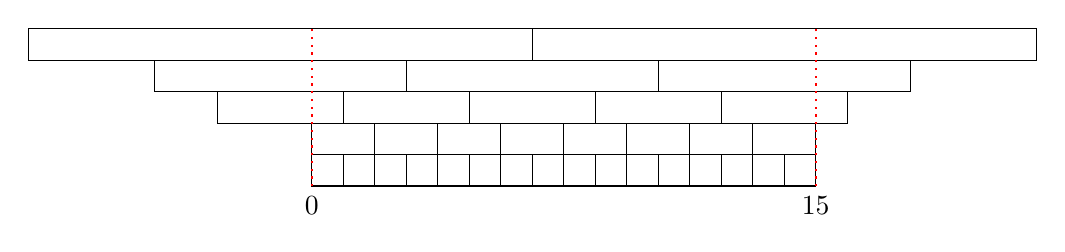
\begin{tikzpicture}[scale=0.4]
  \draw  (0,5) -- (16,5);
  \draw  (-9,4) rectangle (7,5);
  \draw  (7,4) rectangle (23,5);
  \draw  (0,4) -- (16,4);
  \draw  (-5,3) rectangle (3,4);
  \draw  (3,3) rectangle (11,4);
  \draw  (11,3) rectangle (19,4);
  \draw  (0,2) -- (16,2);
  \draw  (-3,2) rectangle (1,3);
  \draw  (1,2) rectangle (5,3);
  \draw  (5,2) rectangle (9,3);
  \draw  (9,2) rectangle (13,3);
  \draw  (13,2) rectangle (17,3);
  
  \draw  (0,3) -- (16,3);
  \draw  (0,1) rectangle (2,2);
  \draw  (2,1) rectangle (4,2);
  \draw  (4,1) rectangle (6,2);
  \draw  (6,1) rectangle (8,2);
  \draw  (8,1) rectangle (10,2);
  \draw  (10,1) rectangle (12,2);
  \draw  (12,1) rectangle (14,2);
  \draw  (14,1) rectangle (16,2);
  
  \draw  (0,1) -- (16,1);
  \draw  (0,0) rectangle (1,1);
  \draw  (1,0) rectangle (2,1);
  \draw  (2,0) rectangle (3,1);
  \draw  (3,0) rectangle (4,1);
  \draw  (4,0) rectangle (5,1);
  \draw  (5,0) rectangle (6,1);
  \draw  (6,0) rectangle (7,1);
  \draw  (7,0) rectangle (8,1);
  \draw  (8,0) rectangle (9,1);
  \draw  (9,0) rectangle (10,1);
  \draw  (10,0) rectangle (11,1);
  \draw  (11,0) rectangle (12,1);
  \draw  (12,0) rectangle (13,1);
  \draw  (13,0) rectangle (14,1);
  \draw  (14,0) rectangle (15,1);
  \draw  (15,0) rectangle (16,1);
  \draw[thick,] node[below] {0} (0,0) -- (16,0) node[below] {15};

  \draw[thick,red, dotted](0,0) -- (0,5);
  \draw[thick,red, dotted](16,0) -- (16,5);
\end{tikzpicture}
\end{center}

\begin{algorithm}
  \Input{query vector \(q\)}
  \Output{}
  \caption{Client Query}
  Retrieve published functions from the server \\
  \((c_1,c_2) \leftarrow f_{query}(f_{encrypt}(f_{bucket}(q)))\) \\
  \While{\(c_2\) is \(False\)} {
    \(q \leftarrow f_{parent}(q)\)\\
    \((c_1,c_2) \leftarrow f_{query}(f_{encrypt}(f_{bucket}(q)))\)
  }
  return \(c_1\)
\end{algorithm}

\section{Motivation}




\end{document}
